% banbe -- what it costs to run (plain-English version of backend-cost-estimate.md)
% Build: tectonic docs/backend-cost-estimate-plain.tex   (or: pdflatex twice)
\documentclass[11pt,a4paper]{article}
\usepackage[margin=18mm,top=16mm,bottom=18mm]{geometry}
\usepackage[T1]{fontenc}
\usepackage[utf8]{inputenc}
\usepackage{helvet}
\renewcommand{\familydefault}{\sfdefault}
\usepackage{xcolor}
\usepackage{tikz}
\usetikzlibrary{positioning,arrows.meta,shapes.misc,fit,backgrounds}
\usepackage{pgfplots}
\pgfplotsset{compat=1.17}
\usepackage[most]{tcolorbox}
\usepackage{booktabs}
\usepackage{array}
\usepackage{enumitem}
\usepackage{amssymb}
\usepackage{hyperref}
\usepackage{microtype}
\usepackage{needspace}

% ---- banbe-like palette ----
\definecolor{paper}{HTML}{F7F4EC}
\definecolor{ink}{HTML}{1B1916}
\definecolor{field}{HTML}{EDE7DA}
\definecolor{gold}{HTML}{C79A2E}
\definecolor{ember}{HTML}{E8572A}
\definecolor{sage}{HTML}{5F7A5A}
\definecolor{sky}{HTML}{3F7CB5}
\definecolor{plum}{HTML}{7A4E8C}
\definecolor{mute}{HTML}{6F6A60}
\pagecolor{paper}
\color{ink}
\hypersetup{colorlinks=true,urlcolor=sky,linkcolor=ink}
\setlength{\parindent}{0pt}
\setlength{\parskip}{6pt}
\setlist{nosep,leftmargin=*}
\pagestyle{empty}

\newcommand{\sectionhead}[1]{\Needspace{15\baselineskip}\vspace{10pt}{\Large\bfseries #1}\par\vspace{-2pt}\textcolor{gold}{\rule{28mm}{2.2pt}}\par\vspace{4pt}}
\newcommand{\bigmoney}[1]{{\fontsize{17}{19}\selectfont\bfseries #1}}

\tcbset{colback=field,colframe=field,arc=4mm,boxrule=0pt,left=3mm,right=3mm,top=2mm,bottom=2mm}

\begin{document}

% ================= HEADER =================
{\fontsize{30}{34}\selectfont\bfseries What does banbe cost to run?}\par
{\large\color{mute} A plain-English guide for Vietnam and the US \quad|\quad October 2026}\par
\vspace{4pt}
\begin{tcolorbox}[colback=ink,colframe=ink,coltext=paper]
\textbf{The short answer.} A launch version of banbe costs about \textbf{\$70 a month}. A busy one-city app (5,000 monthly users) costs about \textbf{\$130--180}. Even at 100,000 monthly users the servers cost about \textbf{\$1,300--1,700}, \emph{if} text-message codes are bought from a cheap local provider. The photos are the cheapest part of the plan. The one decision that can multiply the bill is \textbf{who sends the phone-verification texts}.
\end{tcolorbox}

% ================= 1. COST BY STAGE =================
\sectionhead{1. Four stages of growth}

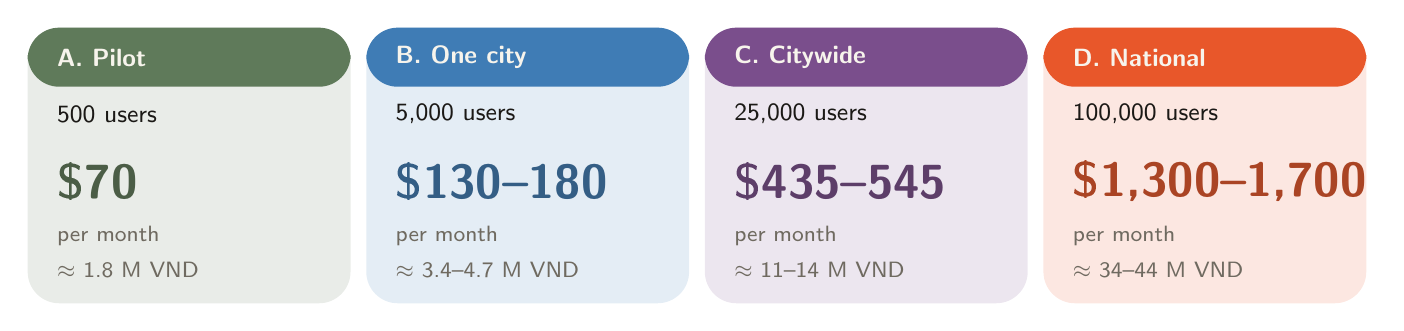
\begin{tikzpicture}[x=1cm,y=1cm]
  \def\w{4.1}
  \foreach \x/\stage/\who/\cost/\vnd/\col in {
    0/A. Pilot/500 users/\$70/1.8 M VND/sage,
    1/B. One city/{5,000 users}/\$130--180/3.4--4.7 M VND/sky,
    2/C. Citywide/{25,000 users}/\$435--545/11--14 M VND/plum,
    3/D. National/{100,000 users}/{\$1,300--1,700}/34--44 M VND/ember}
  {
    \pgfmathsetmacro{\px}{\x*4.3}
    \fill[\col!14,rounded corners=4mm] (\px,0) rectangle (\px+\w,3.5);
    \fill[\col,rounded corners=4mm] (\px,2.75) rectangle (\px+\w,3.5);
    \node[anchor=west,font=\bfseries\small,text=paper] at (\px+0.25,3.12) {\stage};
    \node[anchor=west,font=\small,text=ink] at (\px+0.25,2.4) {\who};
    \node[anchor=west,text=\col!70!ink] at (\px+0.25,1.55) {\bigmoney{\cost}};
    \node[anchor=west,font=\footnotesize,text=mute] at (\px+0.25,0.85) {per month};
    \node[anchor=west,font=\footnotesize,text=mute] at (\px+0.25,0.42) {$\approx$ \vnd};
  }
\end{tikzpicture}

\vspace{2pt}
{\small\color{mute} ``Users'' means \emph{monthly active users}: different people who open the app at least once in a month. Prices in US dollars; 1 USD $\approx$ 26,100 VND. Taxes (VAT) are not included.}

\begin{center}
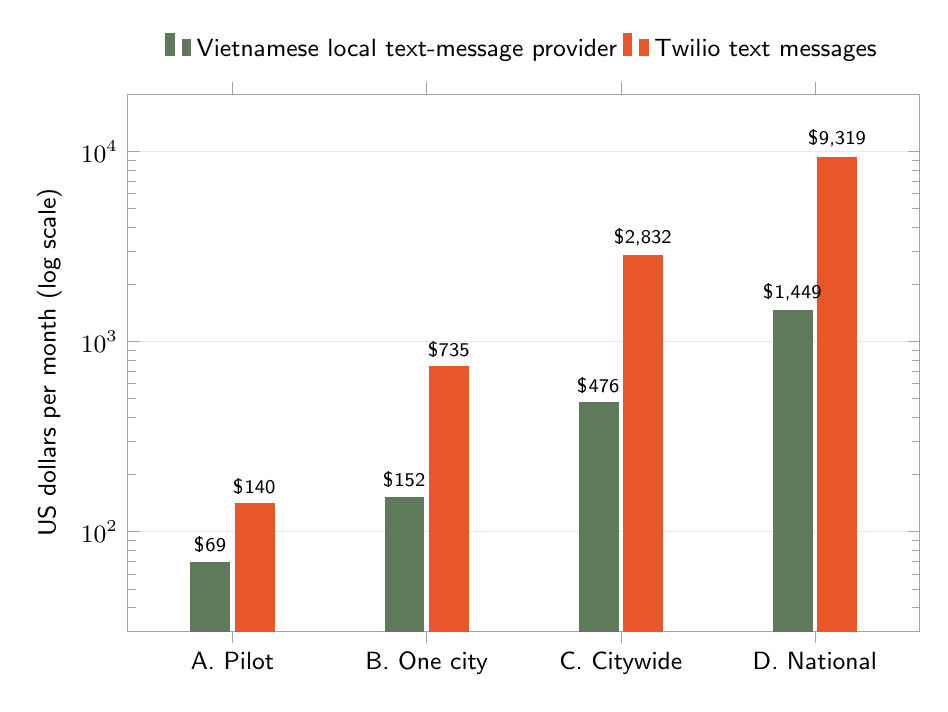
\begin{tikzpicture}
\begin{axis}[
  ybar, bar width=14pt, width=0.96\linewidth, height=8.4cm,
  ymode=log, ymin=30, ymax=20000, log origin=infty,
  symbolic x coords={A. Pilot,B. One city,C. Citywide,D. National},
  xtick=data, enlarge x limits=0.18,
  ylabel={US dollars per month (log scale)}, ylabel style={font=\small},
  yticklabel style={font=\small}, xticklabel style={font=\small},
  nodes near coords={\pgfplotspointmeta}, nodes near coords style={font=\scriptsize,anchor=south},
  legend style={at={(0.5,1.04)},anchor=south,legend columns=-1,draw=none,fill=none,font=\small},
  axis line style={ink!40}, tick style={ink!40}, ymajorgrids, major grid style={ink!10},
]
\addplot[fill=sage, draw=sage, point meta=explicit symbolic] coordinates {(A. Pilot,69) [\$69] (B. One city,152) [\$152] (C. Citywide,476) [\$476] (D. National,1449) [\$1,449]};
\addplot[fill=ember, draw=ember, point meta=explicit symbolic] coordinates {(A. Pilot,140) [\$140] (B. One city,735) [\$735] (C. Citywide,2832) [\$2,832] (D. National,9319) [\$9,319]};
\legend{Vietnamese local text-message provider,Twilio text messages}
\end{axis}
\end{tikzpicture}
\end{center}
{\small\color{mute} The two bars differ only in the price of the verification texts. Everything else is identical.}

% ================= 2. HOW IT IS BUILT =================
\newpage
\sectionhead{2. How banbe is built (the ``hybrid'' plan)}

Think of banbe as a small venue with three rooms. We rent each room from the company that does it best and cheapest.

\begin{center}
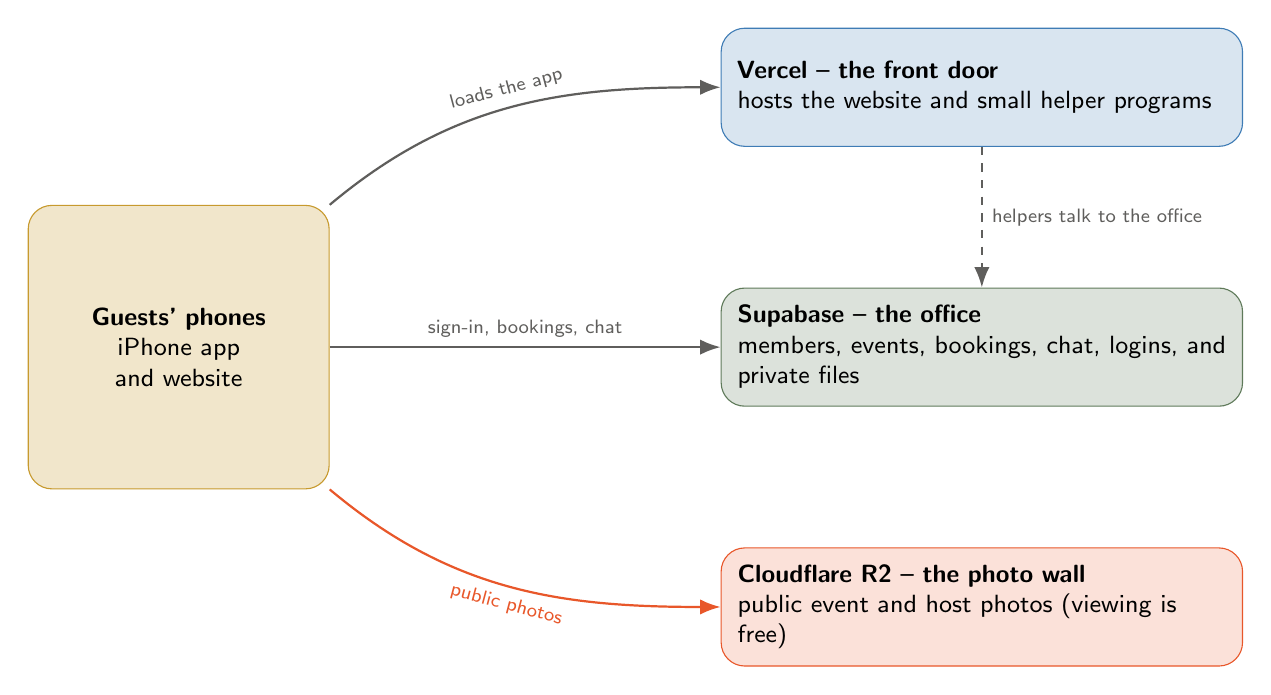
\begin{tikzpicture}[
  every node/.style={font=\small},
  box/.style={rounded corners=3mm,align=left,inner sep=6pt,text width=62mm,minimum height=15mm},
  arr/.style={-{Latex[length=2.6mm]},thick,ink!70}]
  \node[box,fill=gold!25,draw=gold,text width=34mm,align=center,minimum height=36mm] (apps) at (0,0) {\textbf{Guests' phones}\\iPhone app\\and website};
  \node[box,fill=sky!20,draw=sky] (vercel) at (10.2,3.3) {\textbf{Vercel -- the front door}\\hosts the website and small helper programs};
  \node[box,fill=sage!22,draw=sage] (supa) at (10.2,0) {\textbf{Supabase -- the office}\\members, events, bookings, chat, logins, and private files};
  \node[box,fill=ember!18,draw=ember] (r2) at (10.2,-3.3) {\textbf{Cloudflare R2 -- the photo wall}\\public event and host photos (viewing is free)};
  \draw[arr] (apps.north east) to[out=40,in=180] node[above,sloped,pos=0.5,font=\scriptsize]{loads the app} (vercel.west);
  \draw[arr] (apps.east) -- node[above,font=\scriptsize]{sign-in, bookings, chat} (supa.west);
  \draw[arr,ember] (apps.south east) to[out=-40,in=180] node[below,sloped,pos=0.5,font=\scriptsize,text=ember]{public photos} (r2.west);
  \draw[arr,dashed] (vercel.south) -- node[right,font=\scriptsize]{helpers talk to the office} (supa.north);
\end{tikzpicture}
\end{center}

\begin{tabular}{@{}p{34mm}p{54mm}p{74mm}@{}}
\toprule
\textbf{Room} & \textbf{What it does} & \textbf{Why this choice} \\
\midrule
Supabase & Remembers every member, event, booking and chat message; checks logins; keeps private files. & Already built in. Fixed monthly price (\$25) with a generous download allowance. \\
Cloudflare R2 & Stores and shows the public photos. & Downloads are \textbf{free}. Photos are most of what people download, so this keeps the Supabase allowance safe. \\
Vercel & Hosts the website and small helper programs. & Already built in. \$20 a month for commercial use. \\
\bottomrule
\end{tabular}

\begin{tcolorbox}[colback=ember!10,colframe=ember!10]
\textbf{Why not use only Supabase?} It works until photos are downloaded too often. That is what happened in October: the free allowance (5.5 GB) was used up and Supabase paused the app until 12 October. The hybrid plan prevents a repeat and costs almost nothing extra.
\end{tcolorbox}

% ================= 3. WHERE THE MONEY GOES =================
\newpage
\sectionhead{3. Where the money goes}

\begin{center}
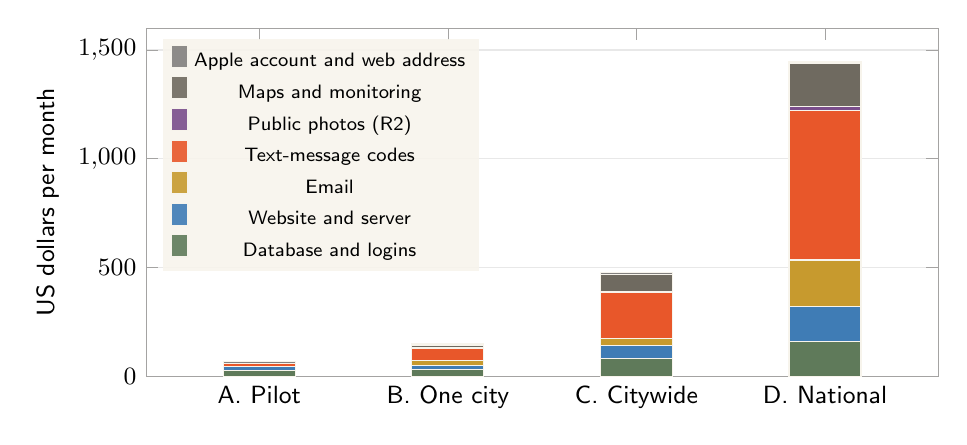
\begin{tikzpicture}
\begin{axis}[
  ybar stacked, bar width=26pt, width=0.96\linewidth, height=6.0cm,
  symbolic x coords={A. Pilot,B. One city,C. Citywide,D. National},
  xtick=data, enlarge x limits=0.2, ymin=0, ymax=1600,
  ylabel={US dollars per month}, ylabel style={font=\small},
  yticklabel style={font=\small}, xticklabel style={font=\small},
  legend style={at={(0.02,0.97)},anchor=north west,font=\scriptsize,draw=none,fill=paper,fill opacity=0.9,text opacity=1,legend columns=1},
  axis line style={ink!40}, tick style={ink!40}, ymajorgrids, major grid style={ink!10},
  reverse legend,
]
\addplot[fill=sage,draw=paper]   coordinates {(A. Pilot,25)  (B. One city,30)  (C. Citywide,80)  (D. National,159)};
\addplot[fill=sky,draw=paper]    coordinates {(A. Pilot,20)  (B. One city,20)  (C. Citywide,60)  (D. National,160)};
\addplot[fill=gold,draw=paper]   coordinates {(A. Pilot,0)   (B. One city,20)  (C. Citywide,35)  (D. National,215)};
\addplot[fill=ember,draw=paper]  coordinates {(A. Pilot,15)  (B. One city,59)  (C. Citywide,211) (D. National,686)};
\addplot[fill=plum,draw=paper]   coordinates {(A. Pilot,0)   (B. One city,2)   (C. Citywide,5)   (D. National,20)};
\addplot[fill=mute,draw=paper]   coordinates {(A. Pilot,0)   (B. One city,12)  (C. Citywide,76)  (D. National,200)};
\addplot[fill=ink!55,draw=paper] coordinates {(A. Pilot,9)   (B. One city,9)   (C. Citywide,9)   (D. National,9)};
\legend{Database and logins,Website and server,Email,Text-message codes,Public photos (R2),Maps and monitoring,Apple account and web address}
\end{axis}
\end{tikzpicture}
\end{center}
{\small\color{mute} Stage B maps/monitoring uses the middle of a \$0--25 range. Totals: A \$69, B \$152, C \$476, D \$1,449.}

\begin{tabular}{@{}p{38mm}p{70mm}p{54mm}@{}}
\toprule
\textbf{Line} & \textbf{In plain words} & \textbf{Cost} \\
\midrule
Database and logins & Supabase Pro plan, plus a bigger ``engine'' as users grow & \$25 $\rightarrow$ about \$160 \\
Website and server & Vercel Pro (required once banbe earns money) & \$20 $\rightarrow$ about \$160 \\
Email & Tickets, receipts and verification emails (Resend) & free $\rightarrow$ about \$215 \\
Text-message codes & A code texted to every new phone number & \textbf{\$15 $\rightarrow$ \$686} (local) or \textbf{\$86 $\rightarrow$ \$8,556} (Twilio) \\
Public photos & Cloudflare R2 storage; viewing is free & \$0 $\rightarrow$ about \$20 \\
Apple account & Needed to publish the iPhone app and tickets in Apple Wallet & \$99 a year (\$8.25 a month) \\
Web address & For example \texttt{media.yourname.com} & about \$12 a year \\
\bottomrule
\end{tabular}

% ================= 4. THE BIG DECISION =================
\sectionhead{4. The one decision that changes the bill: text-message codes}

banbe asks every new member to verify a phone number. Each code is a text message, and the price per text depends heavily on the provider and the country.

\begin{center}
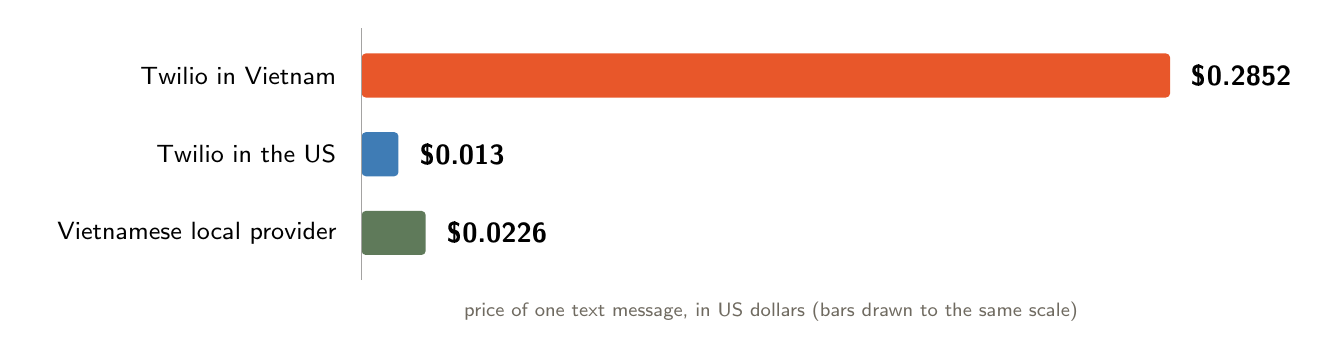
\begin{tikzpicture}[x=1cm,y=1cm,font=\small]
  \def\k{36}% centimetres per US dollar -> 0.2852 USD = 10.3 cm
  \foreach \y/\lab/\val/\col in {2.0/{Twilio in Vietnam}/0.2852/ember, 1.0/{Twilio in the US}/0.013/sky, 0.0/{Vietnamese local provider}/0.0226/sage}
  {
    \pgfmathsetmacro{\len}{\val*\k}
    \node[anchor=east,text width=38mm,align=right] at (-0.2,\y) {\lab};
    \fill[\col,rounded corners=1.5pt] (0,\y-0.28) rectangle (\len,\y+0.28);
    \node[anchor=west,font=\bfseries] at (\len+0.15,\y) {\$\val};
  }
  \draw[ink!40] (0,-0.6) -- (0,2.6);
  \node[anchor=north,font=\scriptsize,text=mute] at (5.2,-0.75) {price of one text message, in US dollars (bars drawn to the same scale)};
\end{tikzpicture}
\end{center}

\begin{tcolorbox}[colback=gold!14,colframe=gold!14]
\textbf{Example, one city (5,000 users, about 2,250 texts a month):} a Vietnamese brandname provider $\approx$ \textbf{\$59}; Twilio in Vietnam $\approx$ \textbf{\$642}. The local price is SpeedSMS's published list (590 VND per text plus a small monthly fee for the registered sender name); other local providers did not show prices, so ask for written quotes. Using a local provider needs a small piece of custom work in Supabase. In the US the standard provider is already cheap (about \$29 a month at this size).
\end{tcolorbox}

% ================= 5. TO DO =================
\newpage
\sectionhead{5. Do we need a separate login service for phone codes?}

\begin{tcolorbox}[colback=sage!16,colframe=sage!16]
\textbf{No.} Supabase already handles the whole login flow. It does not, however, send the text message itself: you must connect \textbf{one} text-message provider behind it. Supabase adds \textbf{\$0} on top of that provider's price, and there is no need for Firebase, Auth0 or Clerk.
\end{tcolorbox}

\begin{center}
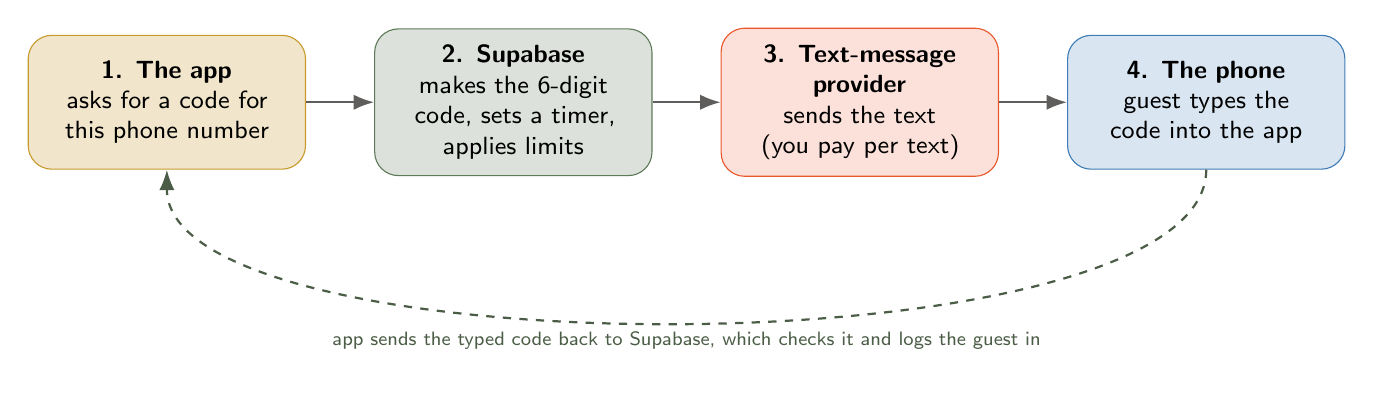
\begin{tikzpicture}[
  every node/.style={font=\small},
  box/.style={rounded corners=3mm,align=center,inner sep=6pt,text width=31mm,minimum height=17mm},
  arr/.style={-{Latex[length=2.6mm]},thick,ink!70}]
  \node[box,fill=gold!25,draw=gold] (app) at (0,0) {\textbf{1. The app}\\asks for a code for this phone number};
  \node[box,fill=sage!22,draw=sage] (sup) at (4.4,0) {\textbf{2. Supabase}\\makes the 6-digit code, sets a timer, applies limits};
  \node[box,fill=ember!18,draw=ember] (sms) at (8.8,0) {\textbf{3. Text-message provider}\\sends the text (you pay per text)};
  \node[box,fill=sky!20,draw=sky] (ph) at (13.2,0) {\textbf{4. The phone}\\guest types the code into the app};
  \draw[arr] (app) -- (sup);
  \draw[arr] (sup) -- (sms);
  \draw[arr] (sms) -- (ph);
  \draw[arr,dashed,sage!70!ink] (ph.south) to[out=-90,in=-90,looseness=0.5] node[below,font=\scriptsize]{app sends the typed code back to Supabase, which checks it and logs the guest in} (app.south);
\end{tikzpicture}
\end{center}

\begin{tabular}{@{}p{58mm}p{52mm}p{46mm}@{}}
\toprule
\textbf{Job} & \textbf{Who does it} & \textbf{Extra cost} \\
\midrule
Make, time-limit and check the code; apply limits; log the guest in & Supabase & included in the \$25 plan \\
Send the text message & A text-message provider you connect & price per text (section 6) \\
Email codes for sign-up and login & banbe's own server (Gmail today) & email service, section 3 \\
Second-step login (``MFA'') by text & Supabase add-on, \textbf{not used by banbe} & \$75 a month, avoid \\
\bottomrule
\end{tabular}

\vspace{6pt}
\textbf{How banbe uses it today.} The phone check happens when a member verifies a phone number (web and iPhone). That is the step that triggers a text. The setting file in the project has the provider switched \emph{off}, but that is only the developer's copy; \textbf{please check the live setting in the Supabase dashboard} (Authentication $\rightarrow$ Providers $\rightarrow$ Phone).

\textbf{Providers.} Supabase has Twilio, Twilio Verify, Bird (MessageBird), Vonage and Textlocal built in. Any other provider (a Vietnamese one, Telnyx, Plivo) connects through a ``send SMS hook'': a small piece of code that receives the code and hands it to the provider. The same hook can deliver by Zalo or email instead.

\textbf{Built-in safety limits.} Supabase allows \textbf{30 texts per hour for the whole project} by default, one code per person every 60 seconds, and 30 code-check attempts per 5 minutes per device. The 30-an-hour cap also limits fraud (at most about \$8.60 an hour on Twilio in Vietnam), but at about 9,000 texts a month (citywide stage) a busy evening could exceed it, so \textbf{raise it as the app grows}. Supabase advises adding a CAPTCHA too; check that your plan offers one.

\begin{tcolorbox}[colback=gold!14,colframe=gold!14]
\textbf{Ways to need fewer texts} (product choices, not priced here): verify the phone only when someone first books or hosts, not at sign-up; offer Zalo or email first in Vietnam with text as backup; skip re-verification on a returning device.
\end{tcolorbox}

\newpage
\sectionhead{6. Text-message providers compared}

Every provider below can send the verification code. They differ in price, in how much fraud protection comes included, and in how easily they plug into Supabase. Prices are per text message in US dollars.

\textbf{Vietnam} (phone numbers starting +84)

{\small
\begin{tabular}{@{}p{37mm}p{30mm}p{91mm}@{}}
\toprule
\textbf{Provider} & \textbf{Price per text} & \textbf{What to know} \\
\midrule
\textcolor{sage}{\textbf{SpeedSMS}} (local) & \textbf{\$0.017--0.030} (450--790 VND) & Published price list. Needs a registered sender name (200,000 VND once, then 200,000 VND a month, about \$7.70). Approval takes 3--5 working days. \\
eSMS, Stringee, VNPT, Viettel (local) & price not shown online & Same kind of service; ask for a written quote. \\
Zalo ZNS & about \$0.008 (200 VND) & Cheap, but only reaches people who use Zalo. Could be the first channel with text messages as backup. \\
\textcolor{sky}{\textbf{Plivo}} & \$0.069--0.228 & Cheapest route is a small carrier; Viettel, the biggest, costs \$0.193. Blended about \$0.157. \\
Bird (MessageBird) & about \$0.155 & Built into Supabase. \\
\textcolor{ember}{\textbf{Twilio}} & \textbf{\$0.2852} & One flat rate, built into Supabase. \\
Firebase & not listed for Vietnam & \$0.01 in the US; needs a billing account. \\
\bottomrule
\end{tabular}}

\vspace{4pt}
\textbf{United States} (phone numbers starting +1)

{\small
\begin{tabular}{@{}p{37mm}p{30mm}p{91mm}@{}}
\toprule
\textbf{Provider} & \textbf{Price per text} & \textbf{What to know} \\
\midrule
\textcolor{sage}{\textbf{Telnyx}} & \textbf{about \$0.008} & Lowest price found. Plugs into Supabase through the ``send SMS hook''. \\
Plivo, Sinch, MSG91 & \$0.0065--0.013 & Low prices, no per-verification fee. \\
Firebase & \$0.01 & A few free texts a day. \\
\textcolor{sky}{\textbf{Twilio} (plain text)} & about \$0.013 & Built into Supabase; a safe default. \\
AWS & about \$0.02 & No fraud protection included. \\
\textcolor{ember}{\textbf{Twilio Verify}} & \textbf{\$0.05 + text} (about \$0.07) & Includes fraud protection, but the fee is about six times the text itself. \\
Vonage Verify & about \$0.07 & Similar to Twilio Verify. \\
\bottomrule
\end{tabular}}

\vspace{6pt}
\textbf{What one city (5,000 users) pays each month for verification texts}

\begin{center}
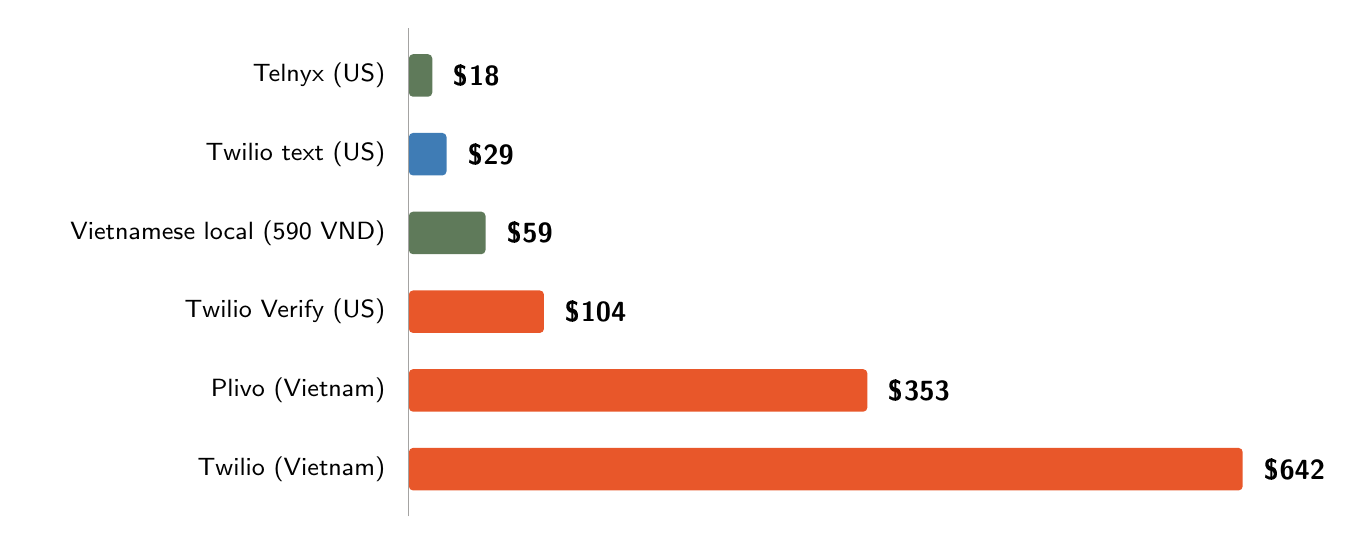
\begin{tikzpicture}[x=1cm,y=1cm,font=\small]
  \def\k{0.0165}% cm per US dollar -> 642 USD = 10.6 cm
  \foreach \y/\lab/\val/\col in {
    5/{Telnyx (US)}/18/sage,
    4/{Twilio text (US)}/29/sky,
    3/{Vietnamese local (590 VND)}/59/sage,
    2/{Twilio Verify (US)}/104/ember,
    1/{Plivo (Vietnam)}/353/ember,
    0/{Twilio (Vietnam)}/642/ember}
  {
    \pgfmathsetmacro{\len}{\val*\k}
    \node[anchor=east,text width=44mm,align=right] at (-0.2,\y) {\lab};
    \fill[\col,rounded corners=1.5pt] (0,\y-0.27) rectangle (\len,\y+0.27);
    \node[anchor=west,font=\bfseries] at (\len+0.15,\y) {\$\val};
  }
  \draw[ink!40] (0,-0.6) -- (0,5.6);
\end{tikzpicture}
\end{center}

\begin{tabular}{@{}p{80mm}rrrr@{}}
\toprule
\textbf{All four stages, per month} & \textbf{A} & \textbf{B} & \textbf{C} & \textbf{D} \\
\midrule
Vietnam: local at 450 VND & \$13 & \$47 & \$163 & \$525 \\
Vietnam: local at 590 VND (used above) & \$15 & \$59 & \$211 & \$686 \\
Vietnam: local at 790 VND & \$17 & \$76 & \$280 & \$916 \\
Vietnam: Plivo & \$47 & \$353 & \$1,413 & \$4,710 \\
Vietnam: Twilio & \$86 & \$642 & \$2,567 & \$8,556 \\
US: Telnyx & \$2 & \$18 & \$72 & \$240 \\
US: Twilio text & \$4 & \$29 & \$117 & \$390 \\
US: Twilio Verify & \$14 & \$104 & \$417 & \$1,390 \\
\midrule
Mixed 70\% Vietnam / 30\% US, cheapest pair & \$11 & \$46 & \$169 & \$552 \\
Mixed 70\% / 30\%, Twilio for both & \$61 & \$458 & \$1,832 & \$6,106 \\
\bottomrule
\end{tabular}

\begin{tcolorbox}[colback=ember!10,colframe=ember!10]
\textbf{Fraud scenario: fake sign-ups.} Bots can request thousands of codes to run up your bill (``SMS pumping''). If 5,000 fake Vietnamese requests arrive in one day, the bill is about \textbf{\$1,426} on Twilio, \textbf{\$785} on Plivo, and about \textbf{\$113} on a Vietnamese local provider (a prepaid balance also caps the loss). The same attack against Twilio in the US costs about \$65. Set limits per phone number, per device and per country, and add a CAPTCHA, from day one.
\end{tcolorbox}

\begin{tcolorbox}[colback=sage!14,colframe=sage!14]
\textbf{Recommendation.} For Vietnamese numbers use a local brandname provider (about 10--15 times cheaper than Twilio). For US numbers use Telnyx or Plivo, or plain Twilio because Supabase supports it directly. Avoid Twilio Verify unless you want its built-in fraud protection. Supabase supports Twilio, Twilio Verify, Bird, Vonage and Textlocal directly, and any other provider through its ``send SMS hook'' (a small piece of custom code).
\end{tcolorbox}

\sectionhead{7. What to do, in order}

\begin{enumerate}[label=$\square$\;,leftmargin=8mm,itemsep=5pt]
\item \textbf{Upgrade Supabase to the Pro plan (\$25).} It fixes the pause immediately; it can be cancelled after a month.
\item \textbf{Move the website to Vercel Pro (\$20)} before launching as a business (the free plan is for non-commercial projects only).
\item \textbf{Choose the text-message providers} (one for Vietnam, one for the US) and get written prices. This is the biggest saving; section 6 compares them.
\item \textbf{Replace Gmail for sending email} with a proper email service (free up to 3,000 emails a month).
\item \textbf{Set up the photo wall (Cloudflare R2) before launch}: buy a web address, shrink the existing photos, then copy them over. One day of work, about \$12 a year.
\item \textbf{Check the live phone-login setting} in the Supabase dashboard, raise the 30-texts-per-hour cap when needed, and turn on a CAPTCHA.
\item \textbf{Check three screens each month:} Supabase usage, Cloudflare R2, and the text-message balance.
\end{enumerate}

% ================= 6. LIMITS =================
\sectionhead{8. How sure are these numbers?}

\begin{tabular}{@{}p{30mm}p{130mm}@{}}
\textbf{Solid:} & Plan prices for Supabase, Vercel, Cloudflare R2, Resend, Twilio, Plivo, Telnyx, SpeedSMS and Apple, read from each company's own page on 9 October 2026. \\[3pt]
\textbf{Estimated:} & How many people use the app, how many photos they view, how many emails and texts are sent, the share of texts going to each phone carrier, the prices of providers whose pages I could not read, and the maps and monitoring costs. \\[3pt]
\textbf{Not included:} & VAT and other taxes; payment fees paid by hosts (Vietnamese bank transfers, Stripe in the US); salaries, legal, and marketing; Vietnamese data-storage rules (ask a lawyer before choosing where the database sits). \\
\end{tabular}

\vspace{8pt}
{\small\color{mute} Full detail, sources and assumptions: \texttt{docs/backend-cost-estimate.md}. Setup steps for Cloudflare R2: note 40 in \texttt{.claude/notes/}.}

\end{document}
